\documentclass[12pt, letterpaper]{report}
\usepackage{graphicx}
\usepackage{titlesec}
\usepackage{wrapfig}
\usepackage{amsmath}
\usepackage[labelfont=bf]{caption}
\usepackage[labelfont=bf]{subcaption}
\begin{document}
\setcounter{secnumdepth}{2}
\titleformat{\chapter}[hang]{\Huge\bfseries}{\thechapter{)}\hspace{20pt}} {0pt}{\Huge\bfseries}
\titleformat{\section}[hang]{\Large\bfseries}{\thesection{)}\hspace{20pt}}{0pt}{\Large\bfseries}
\titleformat{\subsection}[hang]{\large\bfseries}{\thesubsection{)}\hspace{20pt}}{0pt}{\large\bfseries}
	\begin{titlepage}
	
		\begin{center}
		\vspace*{1cm}

		\Large
		\textbf{Physics Engine Workshop Curriculum}\\
		\vspace{2cm}
		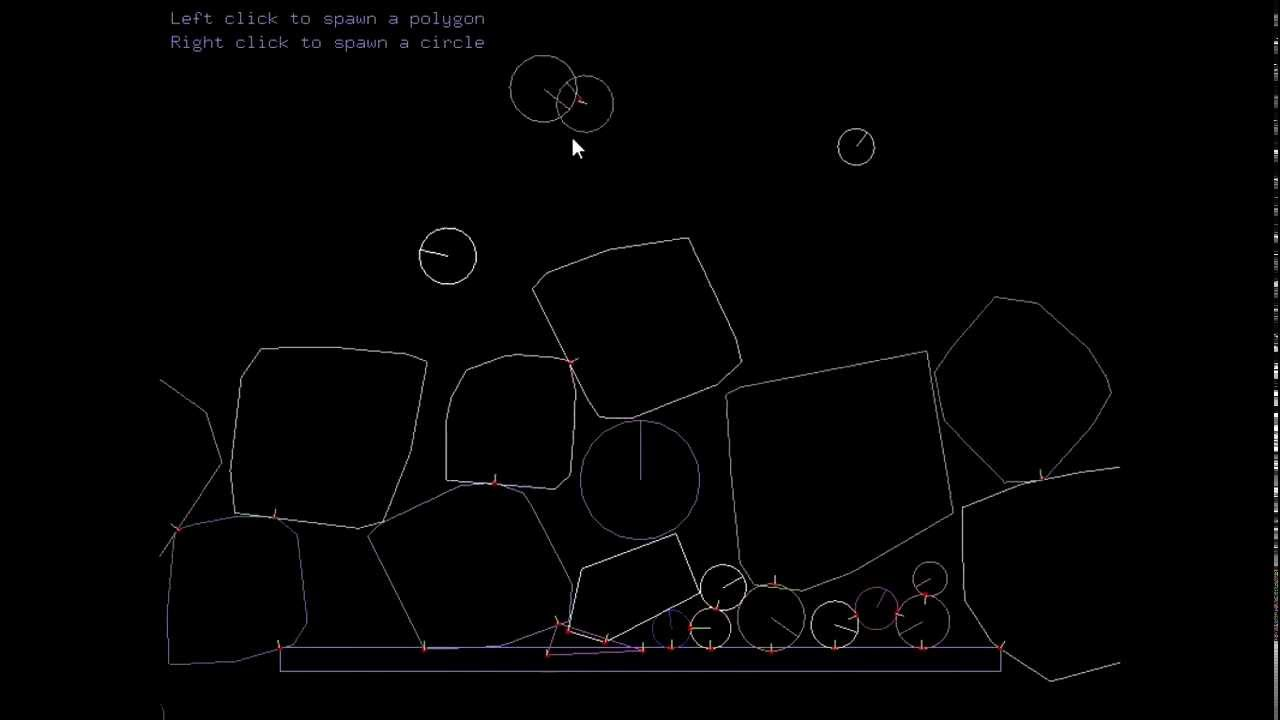
\includegraphics[width=15cm]{Curriculum Images/2dphysics.jpg}\\
		\vspace{2cm}
		\textbf{Great Minds Robotics}\\
		\vspace{1cm}
		\textbf{Austin Long}\\
		\vspace{1cm}
		June 2020\\
		\end{center}
	\end{titlepage}

	\renewcommand{\abstractname}{Workshop Summary}
	\begin{abstract}
		In this workshop we will be exploring the creation of a custom physics engine that we may use towards developing better player interactions, realistic (or non-realistic) movements, and also improve our own understanding of what professional physics engines are actually doing on a more advanced level. We will start by laying the mathematical foundation that we will use to perform all the calculations our engine requires. We will see how the math is directly applicable to even the simplest of games, such as pong and brick breaker, all the way up to advanced monogames with character abilities and environment interaction. A thoroughly fundamental explanation of vectors and their relation to matrices will be provided, with examples on positioning, moving, and rotating multiple shapes. Building on the math, we discuss physical concepts such as momentum, force, acceleration, velocity, mass, gravity, and restitution. Now we set our shapes in motion and let our physics function. Once we have a grasp on how the engine works with a small number of simple objects, we can improve our engine with the application of data structures. The concepts we apply in 2-Dimensions may be expanded into 3-Dimensions, and is the foundation for all professional physics engines. 
	\end{abstract}

\tableofcontents

\renewcommand{\chaptername}{Introduction}
\chapter{Introduction}
	\section{Why a Physics Engine?}
	\paragraph{}Much like in real life, the life in a video game is governed by what we have called physics. Unlike real life however, in a video game, we gain the ability to control the physics within that game. This may sound difficult, but the simple act of bouncing a ball off a paddle is effectively applying some simple knowledge of the physics for object collision. When two objects collide, they may bounce off each other, or stick together, or explode! What determines the result? 
		\subsection{Customization}
		\paragraph{}In a video game, we determine the result. At least if we are willing to create our own engine. We can custom build our engine to have real life characteristics, or have it do something unexpected. We can create ragdoll effects, explosions upon impacts, we can even govern how water and air flow in a 3D world. 
		\subsection{Better Understanding}
		\paragraph{}By creating our own engine, we gain insight in to how a professional physics engine works. We will explore the levels that exist starting from the ground up. By the time we are done, we will have a foundation that can be built upon to build an advanced 2D game focusing around two simple concepts, translation and rotation. The ability to create such an engine is also an excellent method to improve your math, physics, and programming skills.
		\subsection{Appreciability}
		\paragraph{}Finally, we gain an appreciation for what is involved in the creation of such engines. Ours will only deal with simple 2-Dimensional shapes and models, but these engines can be expanded into 3-Dimensions. Our engine depends on the types of physical systems we wish to model, and advanced engines in modern console or PC games involve high levels of math and physics that all build on the foundational concepts of a 2D game. 
	\section{Building Blocks}
	\paragraph{}The math involved can range from anything as simple as arithmetic to as complex as linear algebra or differential calculus. The deciding factor is, what are you trying to model? If we want to model fluid motion, like an ocean, or a stream of water, we need fluid dynamics, which uses differential calculus. If we only want a ball bouncing in the other direction when it collides with an object, we only need arithmetic. If we want the ball to collide with another object, but also collide in a realistic fashion, such as slowing down or changing the proper direction, we need math that is inbetween arithmetic and differential calculus. This math is a branch of linear algebra, and ultimately will use fundamental linear algebra concepts. We are talking about Vector \& Matrix Mathematics. These concepts incorporate arithmetic, algebra, trigonometry, and geometry. Vectors are typically represented in (x, y) point format as they are usually plotted on a graph like the one below.
\vspace{-\baselineskip}
	\begin{figure}[h]
	\centering
	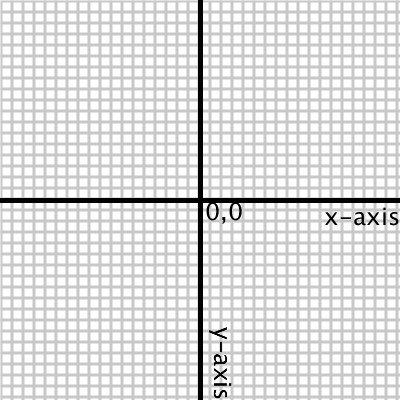
\includegraphics[width=0.5\textwidth]{Processing Images/ConventionalCoordinates/ConventionalCoordinates.jpg}
	\caption{This is a standard coordinate system, otherwise known as an x-y plane. Our origin starts at (0, 0) and is the intersection point of the x and y axes. Every point on the graph may be represented as a pair of x and y points. This is a convention that we use for points and the general format is (x, y).}
	\end{figure}
\newpage
	\paragraph{}The graph itself is also a convention, if we move to the right our x values increase, if we move to the left our x values decrease. Up increases y, down decreases y, but there is nothing that stops us from saying that down may increase y and up may decrease y. A convention is simply something that is widely accepted, and in the programming world the typical convention involves something slightly different than our coordinate system above.
	\section{How a computer draws}
	\paragraph{} Typically when we draw something on an x-y graph, we have our positive x-axis going to the right and our positive y-axis going up. A computer though will draw the x-axis in the same direction, but the y-axis is actually going down. A positive y value will move you farther down the screen while a negative y value will move you up the screen. It is important to gain some practice with this as it will make things easier later. Since computers naturally draw this way, we will be representing everything on our graph as we would see it on our computer screen. 
\\
	\begin{figure}[ht]
	\centering
	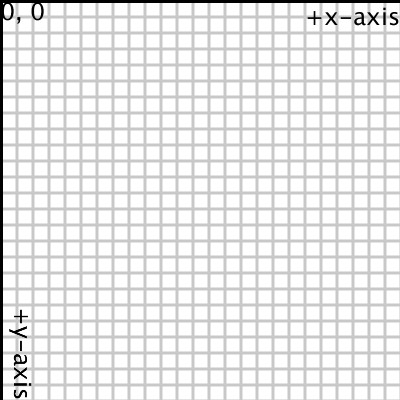
\includegraphics[width=0.5\textwidth]{Processing Images/ComputerAxes/ComputerAxes.jpg}
	\caption{This is the graph our computer will essentially be drawing on. The top left corner is our origin point and this would be the top left corner of the window we have open running our game. As we move to the right, the values along the x-axis are increasing until we reach the full width of our window. As we move down, the values along the y-axis are increasing until we reach the full height of our window.}
	\end{figure}
	\paragraph{} As this takes some practice getting used to, we will be representing all of our shapes and mathematical methods using the above coordinate system. This will hopefully give us enough practice in our way of thinking as a computer would draw and move a shape to make things easier later on.
\chapter{Math}
\paragraph{} Before we start going in to what makes a vector, it is important to ensure that we are all on the same level. This means we are going to cover one of the most useful branches of math that will allow us to understand vectors and essentially any math involving geometry. Trigonometry allows us to describe lengths and angles of shapes in an easy to remember fashion using a few simple rules. 
	\section{Trigs of Trigonometry}
	\paragraph{} Now in order to understand trigonometry, we need to have a basic understanding of algebra. Algebra is where the numbers we have been using in arithmetic start to get replaced with letters. The thing you need to remember is that the letters do not act any different than a regular number. They are simply a placeholder for any number that we may want to plug in to the variable. Algebra also allows us to solve for unknown values given that we know at least two values within an equation. So an equation like $x - 4 = 8$ gives us an x value of 12 by adding 4 to each side of the equation.
	\paragraph{} With trigonometry, we are often dealing with some unknown value in either the x or y directions along with a potentially unknown value for what is called the angle theta, represented by the Greek symbol $\theta$. One of the most common shapes in trigonometry is a triangle, and will be the focus of our work done in this section. The only other shape that is just as common would be a circle, which we will discuss in the following section as it is important to know for rotational motion.
		\subsection{Triangles and You}
		\begin{figure}[h]
		\centering
		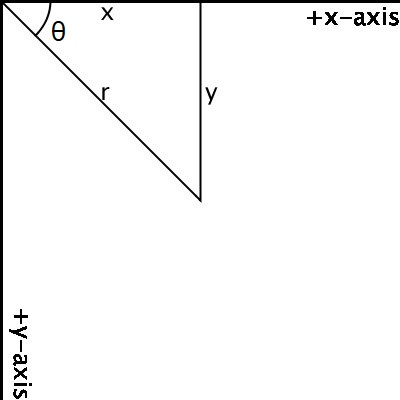
\includegraphics[width=0.5\textwidth]{Processing Images/TrigTri/TrigTri.jpg}
		\caption{A triangle as drawn on a computer screen. The base of the triangle is represented by the value x, the height of the triangle by the value y, and the hypotenuse of the triangle by the value r. The angle the hypotenuse of the triangle makes with the base, or x-axis in this case, is represented by the Greek symbol $\theta$ theta.}
		\end{figure}\vspace{-\baselineskip}
		\paragraph{} In trigonometry, the side next to the angle $\theta$ is called the adjacent side and the side across from the angle $\theta$ is called the opposite side. If we know at least one of these sides, along with the hypotenuse, or both sides in cases where we do not know the hypotenuse, we may solve for the unknown angle theta using the following trigonometric functions:
		\begin{align*}
		sin\left(\theta\right) = \frac{opposite}{hypotenuse} = \frac{y}{r}
		\\\\
		cos\left(\theta\right) = \frac{adjacent}{hypotenuse} = \frac{x}{r}
		\\\\
		tan\left(\theta\right) = \frac{opposite}{adjacent} = \frac{y}{x}
		\end{align*}
		\paragraph{} A useful and rather common method of remembering these equations is by using the phrase known as SOH-CAH-TOA where SOH is just an abbreviation for sine, opposite, hypotenuse and is used to remember that sine is equal to the opposite over the hypotenuse. The same is done for cosine and tangent.
		\paragraph{} Now that we have these relations, we can solve for x, y, or r as long as we know one of those values along with the angle $\theta$. 
		\begin{align*}
		y = rsin\left(\theta\right)\\
		x = rcos\left(\theta\right)\\
		r = \frac{y}{sin\left(\theta\right)} = \frac{x}{cos\left(\theta\right)}
		\end{align*}
It is important to note that the hypotenuse, $r$, has a direct relation to the components x \& y using the following formula:
		\begin{align*}
		r^2 = x^2 + y^2\\
		r = \sqrt{x^2 + y^2}
		\end{align*}
If we do not know the angle, then we may solve for the angle as long as we know two of the sides. This is done using what is known as the inverse trigonometric functions. When we multiply one side of an equation by a value, we must do the same to the other side in order to maintain equality. When we multiply a function with its inverse, the two cancel out and we are left with a variable. Do not worry about understanding why this is the case, as these functions are all derived from infinite sums and series. All that is important is knowing that it works:
		\begin{align*}
		sin^{-1}\left(sin\left(\theta\right)\right) = sin^{-1}\left(\frac{y}{r}\right)
\\	
		\theta = sin^{-1}\left(\frac{y}{r}\right)
		\end{align*}
	The same may be done for cosine and tangent as well. With vectors, tangent is the most commonly used trigonometric function when we are solving for the angle.
	\section{Absolute Unit Circle}
	\paragraph{} Now that we have some familiarity with the foundation of trigonometry, we are going to look at a key piece of the subject that will be incredibly useful for rotating objects. The unit circle is a circle with a radius of one, that we may use to look at how angles change and how these changes affect our x and y values.\\
	\begin{figure}[ht]
	\centering
	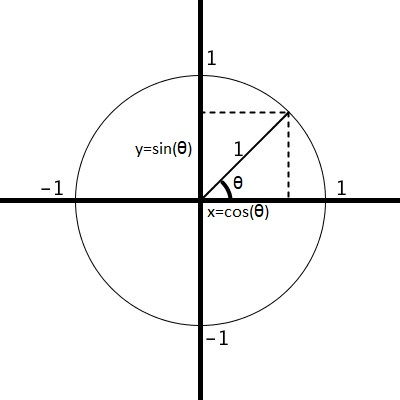
\includegraphics[width=0.5\textwidth]{Processing Images/UnitCircle/UnitCircle.jpg}
	\caption{The radius of a unit circle is constant at a length of one. As we rotate around the circle, the radius remains constant as the angle changes. This angle change causes the value of x to decrease and the value of y to increase as we move from an angle $\theta$ = 0 with x = 1, y = 0 to an angle $\theta$ = 90 degrees with x = 0, y = 1.}
	\end{figure}
	\paragraph{} The unit circle allows us to visualize our lengths and angles in order to see how changes in an angle actually affects the changes in our component length. As long as we maintain the unit circle truth of always having a radius of one, we can see the relation of angular change with our x \& y values. Since we often represent our angles as degrees, we need to cover one last fact about the unit circle. All of the angles in a unit circle are measured using radians. Radians are conventionally related to the number value known as PI ($\pi$) and are usually written as some fraction or multiple of $\pi$. Below we see the same unit circle as above, but this time we write some common angles along the edges of the circle in both degrees and radians for comparison.
	\begin{figure}[ht]
	\centering
	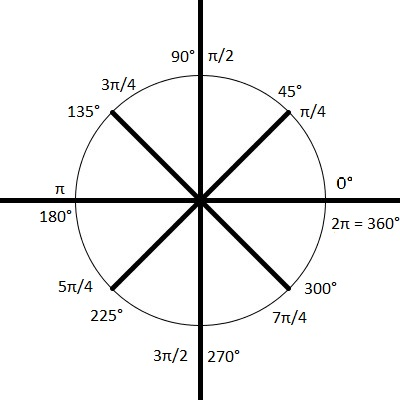
\includegraphics[width=0.5\textwidth]{Processing Images/UnitCircleRadians/UnitCircleRadians.jpg}
	\caption{Here we see equivalence between angles in radians and degrees. Starting off at 0 degrees/radians we may move counter clockwise to 45 degrees, or $\frac{\pi}{4}$ radians. We continue all the way around the circle until we end up back at our starting point. One time, or one cycle, around the circle is equivalent to a 360 degree rotation, also known as $2\pi$ radian rotation.}
	\end{figure}
	\paragraph{} $\pi$ is actually a very important number in math and is used in multiple types of physics based problems, especially involving rotations. The actual value of $\pi$ starts off as 3.14159... and continues on in a non-repeating sequence for an infinite amount of numbers past the decimal. Most programs have a built in $\pi$ value that will be used, but if we ever need to approximate it we will use 3.14159 as this gives us enough accuracy for our purposes. If we ever need to convert between radians and degrees we may use the following relation: 
	\begin{equation*}
	\pi = 180^{\circ}
	\end{equation*}
	\paragraph{} If we want to convert from degrees to radians we will use the ratio $\frac{\pi}{180^{\circ}}$. If we want to convert from radians to degrees we will use the ratio $\frac{180^{\circ}}{\pi}$. This works because after we have moved around our circle $180^{\circ}$ we have gone the equivalent of one $\pi$ radians.
	\paragraph{} Now that we have added some useful tools to our math toolbox, we can start to use them to build an understanding of vectors from the ground up.

\chapter{What is a Vector?}
	\paragraph{}A vector is a way of describing points in space. Vectors may be used to describe the position or motion of a point as well as the distance between points. A vector consists of components which give a vector its magnitude and determine its direction. The magnitude of a vector is simply the length of the vector. It tells us the size of the vector when describing positions or distances. 
	\begin{figure}[h]
	\centering
	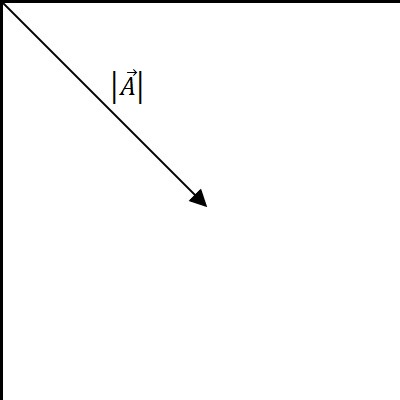
\includegraphics[width=0.5\textwidth]{Processing Images/VectorIntro/VectorIntro.jpg}
	\caption{Here we see a vector as a computer program might draw it. Keeping the origin at the top left corner, the vector length is represented by the symbol $\lvert{\vec{A}}\rvert$ which stands for the magnitude of vector A. The vector itself may be represented as $\vec{A}$ making note of the arrow above the letter, and the $\lvert. \rvert$ are the symbols for magnitude (similar to the absolute value sign).}
	\end{figure}
	\paragraph{} There are two important parts to a vector. We have discussed the first part which is the magnitude or length of the vector. The second part is the direction the vector is pointing. The direction of a vector is described by the angle the vector makes, typically with the x-axis. This is not always the case, as we will see later, we may have an angle between two vectors. For now we will look only at the case for a single vector making an angle $\theta$ with the x-axis.
	\begin{figure}[h]
	\centering
	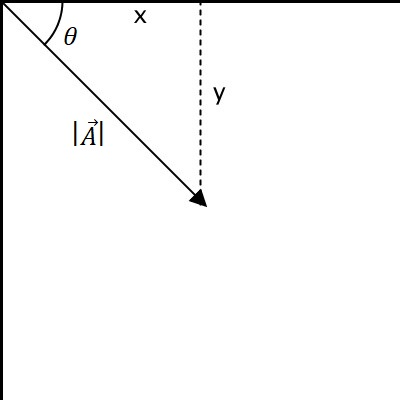
\includegraphics[width=0.5\textwidth]{Processing Images/VectorAngIntro/VectorAngIntro.jpg}
	\caption{Keeping the same layout as a computer would understand it. We can see that our vector $\vec{A}$ makes an angle $\theta$ with the x-axis. Suggestively placing the x \& y symbols along the base and height, we can see that our vector forms a right triangle with our axis. This means that all of the trigonometry we covered in the previous section may be applied directly to our vector.}
	\end{figure}
	\paragraph{} If we want to calculate the magnitude of our vector we may use the same method we used to calculate the length of our hypotenuse. As we were using $r, x,$ and $y$ for our triangle we will substitute to specify we are talking about our vector $\vec{A}$ by using $x$ and $y$ as the subscripts: $A_x$ and $A_y$ for the components, and $\lvert\vec{A}\rvert$ for $r$. This makes the equation for our hypotenuse, which is now the magnitude of our vector $\vec{A}$:
	\begin{equation*}
	\lvert\vec{A}\rvert = \sqrt{A_x^2 + A_y^2}
	\end{equation*}
	\paragraph{} With the methods we discussed in the section on trigonometry, we may find out everything we need to know about our vector $\vec{A}$. If we want the angle $\theta$ we may use the tangent and inverse tangent functions:
	\begin{align*}
	tan\left(\theta\right) = \frac{A_y}{A_x}\\
	tan^{-1}\left(tan\left(\theta\right)\right) = \frac{A_y}{A_x}\\
	\theta = tan^{-1}\left(\frac{A_y}{A_x}\right)
	\end{align*}
	\paragraph{} We may also use the other trig functions to solve for the angle if we happen to know our magnitude. However, the inverse tangent function (sometimes referred to as the arctangent) is the most common approach. If we want to find the components ($A_x$, $A_y$) for our vector, we can use the same method as the last section.
	\begin{align*}
	A_x = \lvert\vec{A}\rvert cos\left(\theta\right)\\
	A_y = \lvert\vec{A}\rvert sin\left(\theta\right)
	\end{align*}
	\paragraph{} Now we have all of the methods we need to analyze a single vector. As you can see, it all originates from trigonometry and triangles. When we go to write a vector out in its official form, it will look like the following:
	\begin{equation*}
	\vec{A} = A_x\hat{i} + A_y\hat{j}
	\end{equation*}
	\paragraph{} Here the symbols $\hat{i}$ and $\hat{j}$ stand for unit vectors. Unit vectors are vectors that have a magnitude of one, and point in the same direction as an x or y axis. $\hat{i}$ is the unit vector along the x-axis and $\hat{j}$ is the unit vector along the y-axis. As these vectors have a magnitude of one, when we multiply them by $A_x$ and $A_y$ respectively, they are scaled by the values of $A_x$ and $A_y$ giving us the components for our vector $\vec{A}$.
	\begin{figure}[ht]
	\centering
	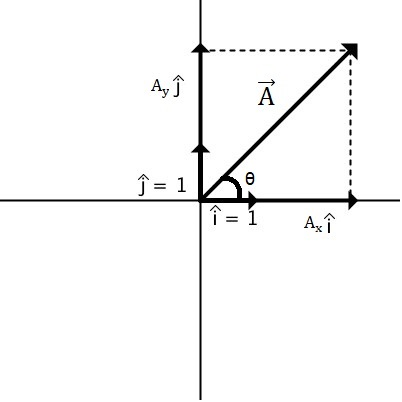
\includegraphics[width=0.5\textwidth]{Processing Images/UnitVector/UnitVector.jpg}
	\caption{Here we see the unit vectors with a unit length of 1 as drawn from the origin. The intersection, or point at which the unit vectors cross each other, occurs at the origin point on the graph. The scaling of these two vectors by $A_x$ $\&$ $A_y$ give us the components for our vector $\vec{A}$. We have drawn this in a typical coordinate system in order to emphasize the scaling of the unit vectors. In a computer program, these axes are treated as a program treats them with the unit vectors running along the axes as shown in this image except with $\hat{j}$ pointing down instead of up.}
	\end{figure}
\newpage
	\paragraph{} Connecting the idea of a vector to real life applications, in real life, you will never actually see a vector. As a vector, like most math, is a modeling construct that we may use to describe an objects momentum, velocity, acceleration, force, flow, position, rotation, among other things. Everything in space may be treated as a single point, moving along some path, that path being described by a vector. When applying vectors to objects, it is important to keep in mind where you set your origin. This will determine where you make your measurements, and to which axis you make your angles. Next we will see how to handle systems with more than one vector. This brings us closer to our goal, as all systems in real life and in programming will typically have more than one object which means more than one vector.

	\section{Vector Algebra}

	\paragraph{} When working with more than one vector, we often want to know where those vectors are in relation to each other. How far apart they are, what is the angle between the vectors, and how much of one vector is ``projected'' on to the other, are some typically useful pieces of information to know. Fortunately there are methods for calculating these pieces of information that build upon the foundation of a single vector. These methods are referred to as vector algebra, and are a fundamental branch of linear algebra as we will see later.
		\subsection{Vector Addition}
		\paragraph{} Let's say we have two vectors as shown in the figure below. We may add these two vectors together, giving us a third vector that we will call vector $\vec{C}$.\vspace{-\baselineskip}
		\begin{figure}[h]
			\centering
			\begin{subfigure}{0.5\textwidth}
			\centering
			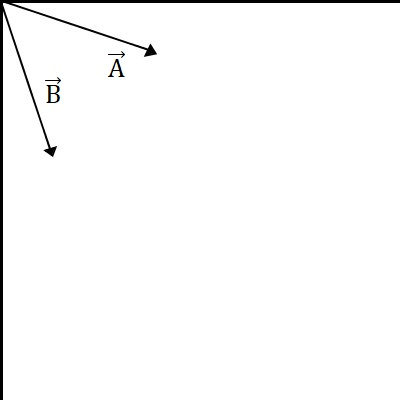
\includegraphics[width=0.75\textwidth]{Processing Images/VectorAddition/Two Vectors.jpg}
			\caption{Here we see vectors $\vec{A}$ \& $\vec{B}$ pointing in different directions with relatively the same magnitude.}
			\end{subfigure}\hspace{0.15cm}
			\begin{subfigure}{0.45\textwidth}
			\vspace{2.5\baselineskip}
			\centering
			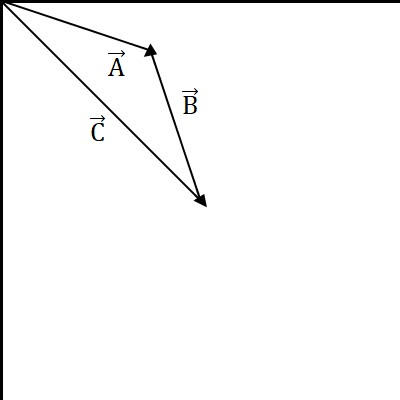
\includegraphics[width=0.75\textwidth]{Processing Images/VectorAddition/VectorAddition.jpg}
			\caption{When we add vectors together graphically, we take the tail of the second vector (tail being its start point) and fix it to the head of the first vector. Drawing another vector from the tail of $\vec{A}$ to the head of $\vec{B}$, we create our third vector $\vec{C}$.}
			\end{subfigure}
		\end{figure}
		\paragraph{} The above shows how we would graphically add two vectors together. Mathematically though, what we end up doing is adding the components of each vector together. We add $A_x$ \& $B_x$ along with $A_y$ \& $B_y$ to create the components of $\vec{C}$. 
		\begin{align*}
		\vec{C} = \vec{A} + \vec{B}\\
		\vec{C} = C_x\hat{i} + C_y\hat{j}\\ where\\
		C_x = A_x + B_x\\
		C_y = A_y + B_y
		\end{align*}
		\paragraph{} This gives us a vector $\vec{C}$ that is subject to all the previously discussed mathematical methods. We may reverse a vectors direction by multiplying it by negative one, which reverses both components of the vector. 
		\begin{figure}[h]
		\centering
		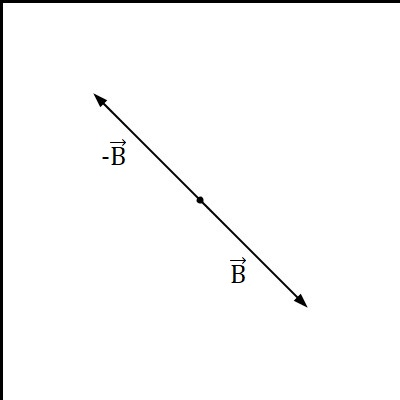
\includegraphics[width=0.5\textwidth]{Processing Images/VectorAddition/NegVector.jpg}
		\caption{Here we have a vector $\vec{B}$ that is pointing down and to the right. When we take the negative of that vector, we flip both the x \& y components. This gives us a vector pointing in the opposite direction, in this case up and to the left. Mathematically, $\vec{B} = B_x + B_y$ becomes $-\vec{B} = -B_x - B_y$.}
		\end{figure}
		\paragraph{} This is useful because often times we want to know how far apart objects are from each other. We can actually describe the distance between objects as a vector, and rather than adding the vectors together we must subtract the vectors. However, subtracting is no different than simply adding a negative value. So our vector $\vec{C}$ becomes $\vec{C} = \vec{A} + (-\vec{B}) = \vec{A} - \vec{B}$. Graphically this looks like the following.
		\begin{figure}[h]
		\begin{subfigure}{0.5\textwidth}
		\centering
		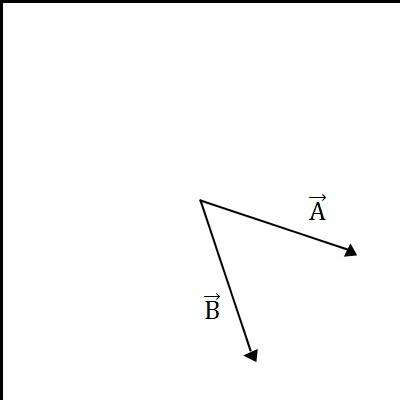
\includegraphics[width=0.5\textwidth]{Processing Images/VectorAddition/2Vect.jpg}
		\caption{Here we start off with two vectors $\vec{A}$ \& $\vec{B}$ this time shifted from the origin for clarity.}
		\end{subfigure}\hspace{0.15cm}
		\begin{subfigure}{0.5\textwidth}
		\centering
		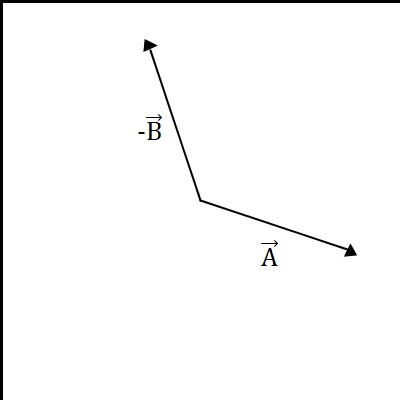
\includegraphics[width=0.5\textwidth]{Processing Images/VectorAddition/2VecNeg.jpg}
		\caption{We start our vector subtraction by first taking the negative of our vector we wish to subtract, in this case $\vec{B}$.}
		\end{subfigure}
		\begin{subfigure}{0.5\textwidth}
		\centering
		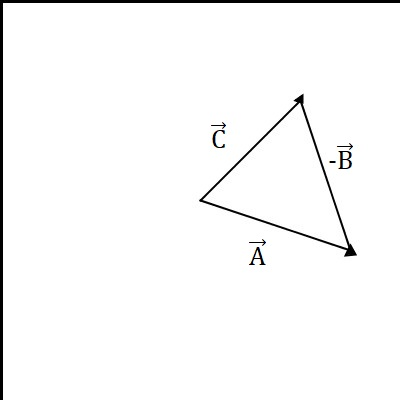
\includegraphics[width=0.5\textwidth]{Processing Images/VectorAddition/2VecSub.jpg}
		\caption{We then perform the same addition method as we did before, placing the tail of our negative vector $\vec{B}$ at the head of our $\vec{A}$ and then drawing our new vector $\vec{C}$ from the tail of $\vec{A}$ to the head of $\vec{B}$.}
		\end{subfigure}
		\end{figure}
		
		\paragraph{} This may not look like it is the distance between vectors $\vec{A}$ and $\vec{B}$, but if we were to compare this to the distance formula:
		
		\begin{equation*}
		Distance = \sqrt{\left(x_2 - x_1\right)^2 + \left(y_2 - y_1\right)^2}
		\end{equation*}
		
		\paragraph{} In words, this means the distance between two points is the square root of the difference between each x point, squared, plus the difference between each y point, squared. Making the substitution for the x and y values using our components of $\vec{A}$ and $\vec{B}$ we get the following:

		\begin{equation*}
		Distance = \sqrt{\left(A_x - B_x\right)^2 + \left(A_y - B_y\right)^2}
		\end{equation*}
		
		\paragraph{} If we consider that $\vec{C} = \vec{A} - \vec{B}$ we may see that the components of $\vec{C}$ are $C_x = A_x - B_x$ and $C_y = A_y - B_y$ and make the following substitution in our equation:

		\begin{align*}
		Distance = \sqrt{\left(C_x\right)^2 + \left(C_y\right)^2}\\
		\lvert\vec{C}\rvert = \sqrt{\left(C_x\right)^2 + \left(C_y\right)^2}
		\end{align*}

		Now we have the magnitude of our vector $\overrightarrow{C}$, and can see that it is in fact the distance between the end point of vector $\vec{A}$ and vector $\vec{B}$. We have now answered the question of how far apart are our vectors. Now what about the angle between the two vectors?
		
		\section{The Dot Product}

		\paragraph{} Before we get in to the method behind finding the angle $\theta$ between our vectors, it is important to understand what a dot product actually is and what it is mathematically doing. A geometric approach to the dot product means that we are taking a projection of a vector upon another vector or axis. Believe it or not, you've encountered projections of a vector before. The components of a single vector starting at the origin, are projections of that vector upon the respective axis. The component $A_x$ is the projection of the vector $\vec{A}$ upon the x-axis, and the component $A_y$ is the projection of the vector $\vec{A}$ upon the y-axis. This means that a projection of a vector is just how much of that vector covers a given region or distance relative to a unit vector. 
		\begin{figure}[ht]
		\centering
		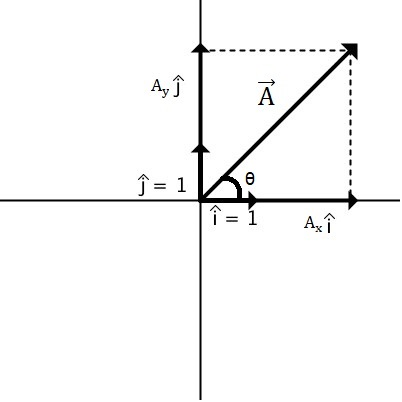
\includegraphics[width=0.5\textwidth]{Processing Images/UnitVector/UnitVector.jpg}
		\caption{We have seen this image before in the last section. Taking a second look now that we have an idea as to the projection of vector $\vec{A}$, we can see that the dashed line going straight up and down represents the projection of the vector on to the x-axis and gives us our x-component, $A_x$. The same may be said for the dashed horizontal line showing the projection of $\vec{A}$ on to the y-axis giving us our y-component $A_y$.}
		\end{figure}
\newpage
		\paragraph{} The mathematical definition for a dot product between vectors $\vec{A}$ and $\vec{B}$ gives us the projection of vector $\vec{A}$ on to the vector $\vec{B}$. 
		\begin{equation*}
		\vec{A}\cdot\vec{B} = \lvert\vec{A}\rvert\lvert\vec{B}\rvert cos\left(\theta\right)
		\end{equation*}
		\paragraph{} The relationship to the angle between the vectors is clearly shown and if we use our unit vector $\vec{i}$ in place of vector $\vec{B}$ we will see how the x-component of vector $\vec{A}$ originates from the projection of $\vec{A}$ on to the unit vector $\vec{i}$ along the x-axis.
		\begin{align*}
		\vec{A}\cdot\vec{i} = A_xi + 0 = \lvert\vec{A}\rvert\lvert\vec{i}\rvert cos\left(\theta\right) \\
		\vec{A}\cdot\vec{i} = A_x = \lvert\vec{A}\rvert cos\left(\theta\right)
		\end{align*}

		\paragraph{} It is important to keep in mind when looking at the equation above that the unit vector $\vec{i}$ has a magnitude of one and has no y-component. If we wanted to find the y-component for our vector $\vec{A}$ we could perform the same operation with the unit vector $\vec{j}$. However, we must keep our angle in mind along with the magnitude of j.
		\begin{align*}
		\vec{A}\cdot\vec{j} = 0 + A_yj=\lvert\vec{A}\rvert\lvert\vec{j}\rvert cos\left(90-\theta\right)\\
		\vec{A}\cdot\vec{j} = A_y = \lvert\vec{A}\rvert cos\left(90 - \theta\right)
		\end{align*}
		\paragraph{} Why did we have to take the difference between 90 degrees and our angle $\theta$? If you look back up at the image, our angle is between the x-axis and unit vector $\vec{i}$ and we may only take a projection of a vector using the angle made by that vector and the axis we wish to project upon. So for the y-component of $\vec{A}$ we actually need to use the angle the vector makes with respect to the y-axis, and that is done by taking the difference between 90 degrees and our x-axis angle, $\theta$. \textbf{Note:} $cos\left(90 - \theta\right) = sin\left(\theta\right)$ as cosine and sine are what we call shifted from each other by 90 degrees. So for example if we use an angle $\theta = 0$ degrees we get $cos\left(90\right)=sin\left(0\right)=0$. This is why $A_y = \lvert\vec{A}\rvert sin\left(\theta\right) = \lvert\vec{A}\rvert cos\left(90-\theta\right)$
		\paragraph{} Before we return to our two vector system, let's look at one more thing the dot product may tell us about our vector $\vec{A}$. If we were to take the dot product of a vector with itself, what would we get? Think of it as we are projecting the vector on to itself, so it's angle $\theta$ would be zero. Mathematically, we would get the following.
		\begin{align*}
		\vec{A}\cdot\vec{A} = \lvert\vec{A}\rvert\lvert\vec{A}\rvert cos\left(0\right)\\
		\vec{A}\cdot\vec{A} = \lvert\vec{A}\rvert^2
		\end{align*}
		\paragraph{} Now we know that when we take the dot product of a vector with itself, we get the magntiude of that vector squared. Well we proved earlier that the magnitude of our vector is $\lvert\vec{A}\rvert = \sqrt{A_x^2 + A_y^2}$ and when we square both sides we get:
		\begin{align*}
		\lvert\vec{A}\rvert^2 = A_x^2 + A_y^2\\
		\lvert\vec{A}\rvert^2 = A_xA_x + A_yA_y
		\end{align*}
		\paragraph{} We now have two relations we can pull from these equations. The first is that we may use the dot product to find the magnitude of a vector by saying that $\lvert\vec{A}\rvert = \sqrt{\vec{A}\cdot\vec{A}}$ and $\vec{A}\cdot\vec{A} = A_xA_x + A_yA_y$. The first relation will be useful for creating our own unit vectors, the second relation will be useful in expanding on our definition of a dot product. Looking back at our original definition:
		\begin{equation*}
		\vec{A}\cdot\vec{B}=\lvert\vec{A}\rvert\lvert\vec{B}\rvert cos\left(\theta\right)
		\end{equation*}
		We may add the relation we just proved to our definition for a dot product.
		\begin{equation*}
		\vec{A}\cdot\vec{B} = A_xB_x + A_yB_y
		\end{equation*}
As A=A, we may also say $\vec{A}\cdot\vec{B}=\vec{A}\cdot\vec{B}$: 
		\begin{equation*}
		\lvert\vec{A}\rvert\lvert\vec{B}\rvert cos\left(\theta\right) = A_xB_x + A_yB_y
		\end{equation*}
We now have a connection between the vector magnitudes, angles, and components. 
		\begin{figure}[ht]
		\centering
		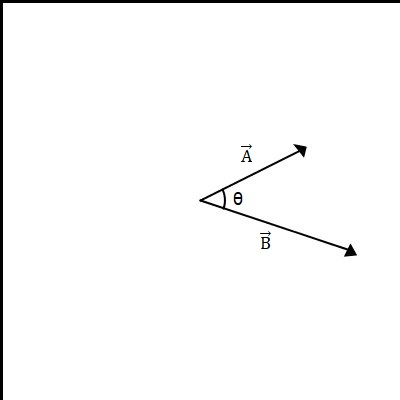
\includegraphics[width=0.5\textwidth]{Processing Images/VectorDotProduct/VectorDotProduct.jpg}
		\caption{}
		\end{figure}
		\paragraph{} If we look back now at our two vector system $\vec{A}$ and $\vec{B}$ we have an angle $\theta$ between the two vectors. We may use the dot product in order to find the angle made between the two vectors. Graphically we have the following: 

		\begin{figure}[h]
		\centering
		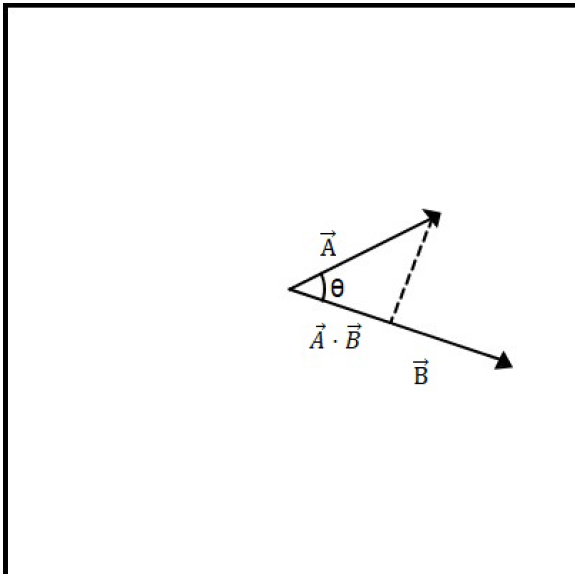
\includegraphics[width=0.5\textwidth]{Curriculum Images/Vectors/Dot Product/ADotProjB.png}
		\caption{Here we graphically see the dot product of $\vec{A}\cdot\vec{B}$ represented as the projection of vector $\vec{A}$ on to the vector $\vec{B}$. This effectively means, how much of vector $\vec{A}$ exists on vector $\vec{B}$.}
		\end{figure}
		\paragraph{} If we take the above equations and rearrange them, we obtain the following solution for the angle between our vectors.
		\begin{align*}
		cos\left(\theta\right)=\frac{A_xB_x+A_yB_y}{\lvert\vec{A}\rvert\lvert\vec{B}\rvert}\\
		\theta = cos^{-1}\left(\frac{A_xB_x+A_yB_y}{\lvert\vec{A}\rvert\lvert\vec{B}\rvert}\right)
		\end{align*}
As long as we know our vector components and magnitudes, we may find the angle that exists between the two vectors. This will be useful later when we get in to collision detection phases and determining true distances between objects.
		\paragraph{}We now have the distance between two vectors, and the angle that is formed between two vectors. This allows us to find out how far away points may be in space along with how much of one vector exists, or is projected on to another vector. This is essential for when we not only want to know the distance between the sides but also distances between corners and edges, or corners and corners. It is also essential for any game physics, as we are subject to the built in global axis of the program such as winforms or monogame, we must in effect project all of our vectors on to the global axis in our solution methods for object collision. Before we do that though, we must project on to their shared axis, which we will see later. For now, we must diverge a bit from our explanation of vectors and see how we may represent vectors in matrix form. This leads us in to fundamental linear algebra topics, which we must use when we are programming our vector system and performing operations on our vector space.

	\chapter{Vectors as Matrices}
	\paragraph{} In the last chapter, it was mentioned that vectors are a part of fundamental concepts in linear algebra. We now cross the bridge in to this realm of linear algebra as we begin to represent our vectors in matrix form. Let us start by asking a question.

		\section{What is a matrix?}
		\paragraph{} We may think of a matrix as a collection of values, in our case numbers. They are represented in a row by column format such as 2x2 or 3x3 or 2x3 etc. In fact, we may even think of a single number as a 1x1 matrix. Below are some examples of various matrices.

		\begin{equation*}
		\begin{bmatrix}
		1 
		\end{bmatrix}
\\
		\begin{bmatrix}
		1 & 2\\
		3 & 4
		\end{bmatrix}
\\
		\begin{bmatrix}
		11 & 12\\
		21 & 22\\
		31 & 32
		\end{bmatrix}
		\end{equation*}
		
		\paragraph{} As we move from left to right, the matrices all represent a 1x1, 2x2, and 3x2 matrix, respectively. The dimensions of the matrix are listed in a row x column or rxc format. The values of the matrix on the right represent the index of the element for the matrix. Each element is found as a row-column index, and we may define a generic 2x2 matrix A.

		\begin{equation}
		\begin{bmatrix}
		A
		\end{bmatrix}
		=
		\begin{bmatrix}
		A_{11} & A_{12}\\
		A_{21} & A_{22}
		\end{bmatrix}
		\end{equation}
		
		\paragraph{} It is tempting to immediately say that this matrix represents our vector $\vec{A}$, but recall our vector only has two points describing it. Any two points on an x-y plane may be represented as a single 2x1 matrix.
		\begin{equation*}
		\begin{bmatrix}
		x\\
		y
		\end{bmatrix}
		\end{equation*}
		This means we may represent our vector $\vec{A}$ in matrix form as follows:
		\begin{equation*}
		\begin{bmatrix}
		A
		\end{bmatrix}
		=
		\begin{bmatrix}
		A_x\\
		A_y
		\end{bmatrix}
		\end{equation*}
		\paragraph{} Now we must ensure that all of our math that we applied to vectors is still applicable to our matrix. In some cases, it is even easier to perform our vector math using matrices, as we will see in the next section.
		\section{Matrix math}
		\paragraph{} The process of performing math operations with matrices is fairly straight forward. If we have two matrices A and B and we want to add them together, all we need to do is add the elements of each matrix together. Subtraction works the same way, however, when we get to multiplication and division things get a little more complicated. In order to divide one matrix by another matrix, we must perform the inverse on the dividing matrix, and then multiply that now inversed matrix with the other matrix we wish to divide. This is not always possible as not all matrices have an inverse, and fortunately for us is not required in order to build out a simple engine. One thing that is required though is knowing how to multiply two matrices together, as the multiplication of two matrices is equivalent to the dot product of two vectors, we will be performing this operation quite often.
		\subsection{Matrix multiplication}
		\paragraph{} Matrix multiplication involves the combination of two matrices resulting in one new matrix. The final result leaves us a matrix with dimensions that are a mix of the two matrices being multiplied. This means that if we multiply a 2x2 matrix with another 2x2 matrix, we end up with a 2x2 matrix. If we multiply a 3x2 matrix with a 2x1 matrix, we end up with a 3x1 matrix. If we multiply a 1x3 matrix with a 3x1 matrix, we end up with a 1x1 matrix. What's the pattern?

		\paragraph{} Since the resulting matrix will be a combination of the first two matrices, we must follow one rule in order to actually have the ability to multiply them together. The rule is that we may only multiply matrices that share dimensions, specifically the number of columns in the first matrix must equal the number of rows in the second matrix. The dimensions of the resulting matrix is then equal to the number of rows of the first matrix and the number of columns of the second matrix. There are methods to multiply matrices that do not follow this rule, but we will not explore those as they are more advanced and unnecessary for our purposes.

		\paragraph{} We may represent matrix multiplication with the following notation. Let the general matrix A be a 3x2 matrix and the matrix B be a 2x2 matrix.

		\begin{equation}
		\begin{bmatrix}
		A
		\end{bmatrix}
		\begin{bmatrix}
		B
		\end{bmatrix}
		=
		\begin{bmatrix}
		A_{11} & A_{12}\\
		A_{21} & A_{22}\\
		A_{31} & A_{32}
		\end{bmatrix}
		\begin{bmatrix}
		B_{11} & B_{12}\\
		B_{21} & B_{22}
		\end{bmatrix}
		\end{equation}

		\paragraph{} The resulting matrix has the dimensions 3x2, how do we calculate each element of the new matrix?
 
		\begin{equation*}
		\begin{bmatrix}
		A_{11}B_{11}+A_{12}B_{21} & A_{11}B_{12}+A_{12}B_{22}\\
		A_{21}B_{11}+A_{22}B_{21} & A_{21}B_{12}+A_{22}B_{22}\\
		A_{31}B_{11}+A_{32}B_{21} & A_{31}B_{12}+A_{32}B_{22}
		\end{bmatrix}
		\end{equation*}

		\paragraph{} Each element is calculated using the method shown above, what is the pattern? We take the first row of the first matrix and the first column of the second matrix, we step through multiplying each element together and adding the results until we reach the end of the row and column. This gives us the first element for our new matrix C.

		\begin{equation}
		\begin{bmatrix}
		C
		\end{bmatrix}
		=
		\begin{bmatrix}
		A
		\end{bmatrix}
		\begin{bmatrix}
		B
		\end{bmatrix}\\
		\end{equation}
		\begin{equation*}
		\begin{bmatrix}
		C_{11} & C_{12}\\
		C_{21} & C_{22}\\
		C_{31} & C_{32}
		\end{bmatrix}
		=
		\begin{bmatrix}
		A_{11}B_{11}+A_{12}B_{21} & A_{11}B_{12}+A_{12}B_{22}\\
		A_{21}B_{11}+A_{22}B_{21} & A_{21}B_{12}+A_{22}B_{22}\\
		A_{31}B_{11}+A_{32}B_{21} & A_{31}B_{12}+A_{32}B_{22}
		\end{bmatrix}
		\end{equation*}
\chapter{Linear Transformations}	
	\paragraph{}A linear transformation essentially allows us to transform our matrix without losing the ability to apply addition and scalar multiplication operations to our matrix. This is important because it allows us to modify our matrix without losing the original information. We define two important transformations as the following matrices.

	\section{Translation}
	We may define a 2D translation matrix as follows

	\begin{equation}
	\mathbf
	T = 
	\begin{bmatrix}
	1 & 0 & dx\\
	0 & 1 & dy\\
	0 & 0 & 1
	\end{bmatrix}
	\end{equation}

	\paragraph{} Here dx and dy represent our desired change in the x and y directions respectively. When we apply this matrix to any 2D vector, it will shift that vector by the amounts dx and dy. We apply this matrix by multiplying it with the vector we want to shift. The derivation for the transformation matrix may be found in the appendix. The foundational matrix that allows us to use this translation is the identity matrix and is shown in the appendix derivation.

	\paragraph{} It is important to note that this is a 3x3 matrix. We must therefore apply it to a matrix that has three rows. If we recall our general 2D matrix for a vector was a 2x1 matrix. To convert this to allow us to multiply the two matrices together, we must homogenize our vector in to a 3x1 by making the following change.
	
	\begin{equation}
	\begin{bmatrix}
	A
	\end{bmatrix}
	=
	\begin{bmatrix}
	A_x\\
	A_y\\
	1
	\end{bmatrix}
	\end{equation}
	
	\paragraph{} The addition of one in the third row allows us to maintain a consistent coordinate system without changing our vector. We may think of this as including the magnitude of a unit vector that helps us preserve our coordinate system. 

	\paragraph{} We may now use our translation operator on our vector $\overrightarrow{A}$. When we apply our operator to our vector we get the following.
	
	\begin{align*}
	\mathbf 
	T\overrightarrow{A} 
	&= 
	\begin{bmatrix}
	T
	\end{bmatrix}
	\begin{bmatrix}
	A
	\end{bmatrix}\\
	&=
	\begin{bmatrix}
	1 & 0 & dx\\
	0 & 1 & dy\\
	0 & 0 & 1
	\end{bmatrix}
	\begin{bmatrix}
	A_x\\
	A_y\\
	1
	\end{bmatrix}\\
	&=
	\begin{bmatrix}
	A_x+dx\\
	A_y+dy\\
	1
	\end{bmatrix}
	\end{align*}

	\paragraph{} We have now shifted the components of our vector. If we want to shift our vector back, we can perform the inverse operation as well.
	
	\begin{equation}
	\mathbf
	T^{-1} =
	\begin{bmatrix}
	1 & 0 & -dx\\
	0 & 1 & -dy\\
	0 & 0 & 1
	\end{bmatrix}
	\end{equation}

	\paragraph{} In programming we will often be performing the inverse translation first, then the normal translation. This is because we must shift our objects back to the global origin first, aligning the local and global origins, then perform any changes we need, followed by a normal translation back to the ``original" position.

	\newpage
	\section{Rotation}
	\paragraph{} As we defined a translation matrix, we will define a rotation matrix along the same principles.
	
	\begin{equation}
	\mathbf
	R = 
	\begin{bmatrix}
	\cos{\theta} & -\sin{\theta} & 0\\
	\sin{\theta} & \cos{\theta} & 0\\
	0 & 0 & 1
	\end{bmatrix}
	\end{equation}

	\paragraph{} This works the same way as the translation matrix, however rather than shifting the x and y points, this will rotate each point by some angle $\theta$ relative to the global origin. Applying this to our matrix A gives us the following.
	
	\begin{align*}
	\mathbf
	R\overrightarrow{A} &= \begin{bmatrix}R\end{bmatrix}\begin{bmatrix}A\end{bmatrix}\\
	&=
	\begin{bmatrix}
	\cos{\theta} & -\sin{\theta} & 0\\
	\sin{\theta} & \cos{\theta} & 0\\
	0 & 0 & 1
	\end{bmatrix}
	\begin{bmatrix}
	A_x\\
	A_y\\
	1
	\end{bmatrix}\\
	&=
	\begin{bmatrix}
	A_x\cos{\theta} - A_y\sin{\theta}\\
	A_x\sin{\theta} + A_y\cos{\theta}\\
	1
	\end{bmatrix}
	\end{align*}

	\paragraph{} It is important to keep in mind this performs a rotation about the origin of the global axis. Since the origin for our screen is in the top left corner, this will rotate our object about that origin point. If we want to rotate an object about its center or some other point, we must first translate it to the origin, rotate it, then translate it to where we want it. An inverse rotation matrix is also possible, where we simply use an angle -$\theta$.
\\

	\Huge INSERT IMAGE HERE
	\normalsize

	\paragraph{} We now have the tools we need to translate and rotate any object we desire. With the creation of mathematical functions that can be applied in a translation \& rotation function, we need only store the current position, translate our object, rotate it, then restore the previous position.

\chapter{Broad Phase Collision Detection}
\paragraph{} Now that we are familiar with the mathematical formulations we will be using to move and rotate our shapes, we are going to look at how we can detect the collision between two shapes, and how to respond appropriately. Without proper collision detection our shapes may pass through each other without any effect what so ever and can cause the player's character to fall through the world because if you can't detect the collision with the ground, how do you know it is there?
\paragraph{} We will start off simple of course, with what are called Axis-Aligned Bounding Boxes (AABBs). These are effectively imaginary squares or rectangles that enclose our object in space. We may put any type of shape inside of these boxes to determine what are known as broad phase collisions. These types of collisions simply look at two objects potential for a collision. If the objects are within a certain distance, they could potentially be colliding depending on their true geometric shape. Broad phase collision is the first check to perform when trying to determine whether two or more objects are colliding. 
	\section{Axis-Aligned Bounding Box}
	\paragraph{} In principle, you have most likely created an Axis-Aligned Bounding Box, henceforth referred to as AABB, you just didn't realize that's what it was called. Fundamentally, an AABB is an imaginary box that is created around our shapes. This box acts as a container, and stores minimum and maximum values for our shape. This means that with just a single check, comparing min and max values, we can determine on a broad level whether our shapes are actually colliding. If the AABB of one shape is overlapping with the AABB of another shape, we have a potential collision. 
	\paragraph{}This may be done a couple ways, where the brute force way involves checking all four sides against each other for both shapes. This means one check with four comparisons, returning true or false depending on if you're checking for an overlap or no overlap. A more elegant way is by creating a vector that points to the minimum, or the bottom left point of our rectangle, and a vector that points to the maximum, or the top right point of our rectangle. This allows us to check both the smallest and largest (x, y) point, simplifying our check to only two comparisons. If there is an axis that overlaps between the shapes, we have a collision. Keep in mind, that in most programming languages, the minimum will actually be the top left corner, and the maximum will be the bottom right corner. This is due to the inversion of the y-axis in that it is drawing down instead of up.
	\paragraph{} One key idea to keep in mind comes from the name itself, Axis-Aligned. This means that our AABB can not be rotated relative to each other. Each side of the AABB must be parallel or perpendicular to the global screen axis. This kind of check is primarily for direct collisions, where the centers and sides of each shape are aligned. This does not mean our shape is forbidden from rotating, remember the AABB is just an imaginary box surrounding the shape. However, if our shape is rotating, the dimensions of the box must change accordingly. The box itself will never actually rotate though, in the simplistic form of AABB collisions.
	\section{Bounding Sphere}
	\paragraph{} A bounding sphere is similar to an AABB. Rather than being an imaginary box around an object, a bounding sphere (or bounding circle in 2D) is an imaginary sphere around an object. The center of the object is the center of the circle, and the radius is made from the longest distance across the object in order to encircle the whole thing. Obviously this type of bound is not useful for long or flat objects, as those are typically more rectangular, an AABB would be a better choice. 
	\paragraph{} A few advantages to using a bounding sphere is that our object may rotate without any adjustment of our bound. All we need is to move our sphere with our object and regardless of the objects orientation it is guaranteed to fit within our sphere. This makes computation significantly easier as it removes any resizing that might be needed in the case of an AABB. 
	\paragraph{} In order to determine the distance between two spheres or circles, we simply take the distance between the centers of the object and check to see if it is less than the sum of the radii for our spheres/circles. If the distance is smaller, our objects are most likely colliding or heading towards a collision. Remember, we are still in the broad phase so we are simply looking for possible collisions, not exact collisions.
	\section{The Separating Axis Theorem \& Narrow Phase Detection}
	\paragraph{} After our broad phase detection, we must refine our engine to detect objects at their true size. Highly sophisticated engines use what are called convex and concave meshes to essentially mold a hitbox for any given shape. This creates a mesh layer over the object, typically in 3-Dimensions, that is then used as the narrow phase hitbox for collisions. As objects can be either convex or concave, it may become difficult and quite innaccurate if these shapes are not modeled properly at the physics level. For instance, if we model a concave shape like a bowl using a convex hitbox, our character will have a bowl of levitating fruit or some other object. If we model a convex shape using a concave hitbox, we may end up inside the car, or we may end up inside the cars engine. The geometry of our shape becomes important when we want to accurately model our objects. 
	\paragraph{} We will not be dealing with these mesh types of hitboxes just yet. First we need to check our shapes to see if they are colliding, and in order to do this we need to find our axis that we will be using to separate our shapes. We may think of an axis that we are creating as a vector that is sitting at a 90 degree angle to each side of our shape. We call this axis, or vector, $\hat{n}$ and may treat this as an imaginary local axis relative to our shapes. If we then take the distance between our edge and a point, or vertex, of our other shape, we can project this distance on to our imaginary local axis $\hat{n}$ using the dot product. If this projection is greater than 0, then our objects are not yet colliding. Mathematically, this is represented as:
	\begin{equation*}
	\left(v-a\right)\cdot\hat{n}
	\end{equation*}
Where $v$ is the vertex point of our second shape, and $a$ is some point along the edge of our first shape of which our axis $\hat{n}$ is created.
\end{document}

 